% Copyright (c) 2026 Selina Cheggour. Tous droits réservés. Voir le fichier LICENSE.
% Fiche 2 : séance 1 du TP (parties 0 à 3). Visuelle, sans explications longues : l'encadrante explique à l'oral.
% Les valeurs « Tu dois voir » sont celles des cellules de vérification du notebook.

\newcommand{\doisvoir}[1]{\par\smallskip{\color{accentblue}\faCheckCircle\ \textbf{Tu dois voir :}} #1}
\newcommand{\image}[1]{\par\smallskip{\color{lightblue}\faChild}\ \textit{#1}}

\bandeaupartie{Fiche 2 : séance 1}{Avant d'entraîner quoi que ce soit, on vérifie.}

\section{La séance en une image}

\begin{center}
\begin{tikzpicture}[
  etape/.style={draw=#1, fill=#1!10, rounded corners=6pt, minimum width=3.55cm, minimum height=2.7cm,
    align=center, text width=3.3cm, font=\small},
  fl/.style={-{Stealth[length=3mm]}, very thick, color=slate}]
\node[etape=slate] (p0) {{\huge\faTools}\\[3pt]\textbf{0. Installer}\\corpus, 2 bibliothèques, outils};
\node[etape=sectioncolor, right=0.4cm of p0] (p1) {{\huge\faBoxOpen}\\[3pt]\textbf{1. Vérifier}\\les données sont-elles ce qu'on croit ?};
\node[etape=accentblue, right=0.4cm of p1] (p2) {{\huge\faTag}\\[3pt]\textbf{2. Définir}\\que prédit-on, au juste ?};
\node[etape=darkblue, right=0.4cm of p2] (p3) {{\huge\faBalanceScale}\\[3pt]\textbf{3. Mesurer}\\sans tricher};
\draw[fl] (p0) -- (p1); \draw[fl] (p1) -- (p2); \draw[fl] (p2) -- (p3);
\end{tikzpicture}
\end{center}

\begin{enfant}
\textbf{Comme une recette de gâteau} : vérifier que le sachet \og sucre \fg{} contient du sucre,
choisir quel gâteau, et décider comment on saura s'il est réussi. \emph{Avant} d'allumer le four.
\end{enfant}

\section{Partie 0 : mise en route}

\begin{stepbox}[title={\faPlay\quad Exécute les 3 cellules, sans rien modifier}]
\begin{tabularx}{\linewidth}{>{\bfseries\color{sectioncolor}}c X}
0.1 & \faDownload\ télécharge le corpus : environ 650 Mo, 3 Go sur le disque. Quelques minutes, sans affichage. \\
0.2 & \faPuzzlePiece\ installe \texttt{opensmile} (la voix) et \texttt{jiwer} (les erreurs de transcription). \\
0.3 & \faToolbox\ charge les outils du TP, dont \texttt{verifier}. \\
\end{tabularx}
\doisvoir{\texttt{1446 appels disponibles}, puis \texttt{Outils chargés.} et la liste des versions.}
\end{stepbox}

\begin{tcbraster}[raster columns=2, raster equal height, raster column skip=8pt, raster every box/.style={unbreakable}]
\begin{enfant}[unbreakable]
\texttt{/kaggle/working} = le \textbf{cartable}, pesé à chaque sauvegarde.
\texttt{/kaggle/temp} = la \textbf{table}, nettoyée le soir. Le corpus va sur la table.
\end{enfant}
\begin{enfant}[unbreakable]
\texttt{[À revoir]} = la maîtresse écrit \og à revoir \fg{} dans la marge, avec un
\textbf{indice}, au lieu de déchirer la copie. Lis l'indice !
\end{enfant}
\end{tcbraster}

\section{Partie 1 : contrôle à la réception}

\begin{center}
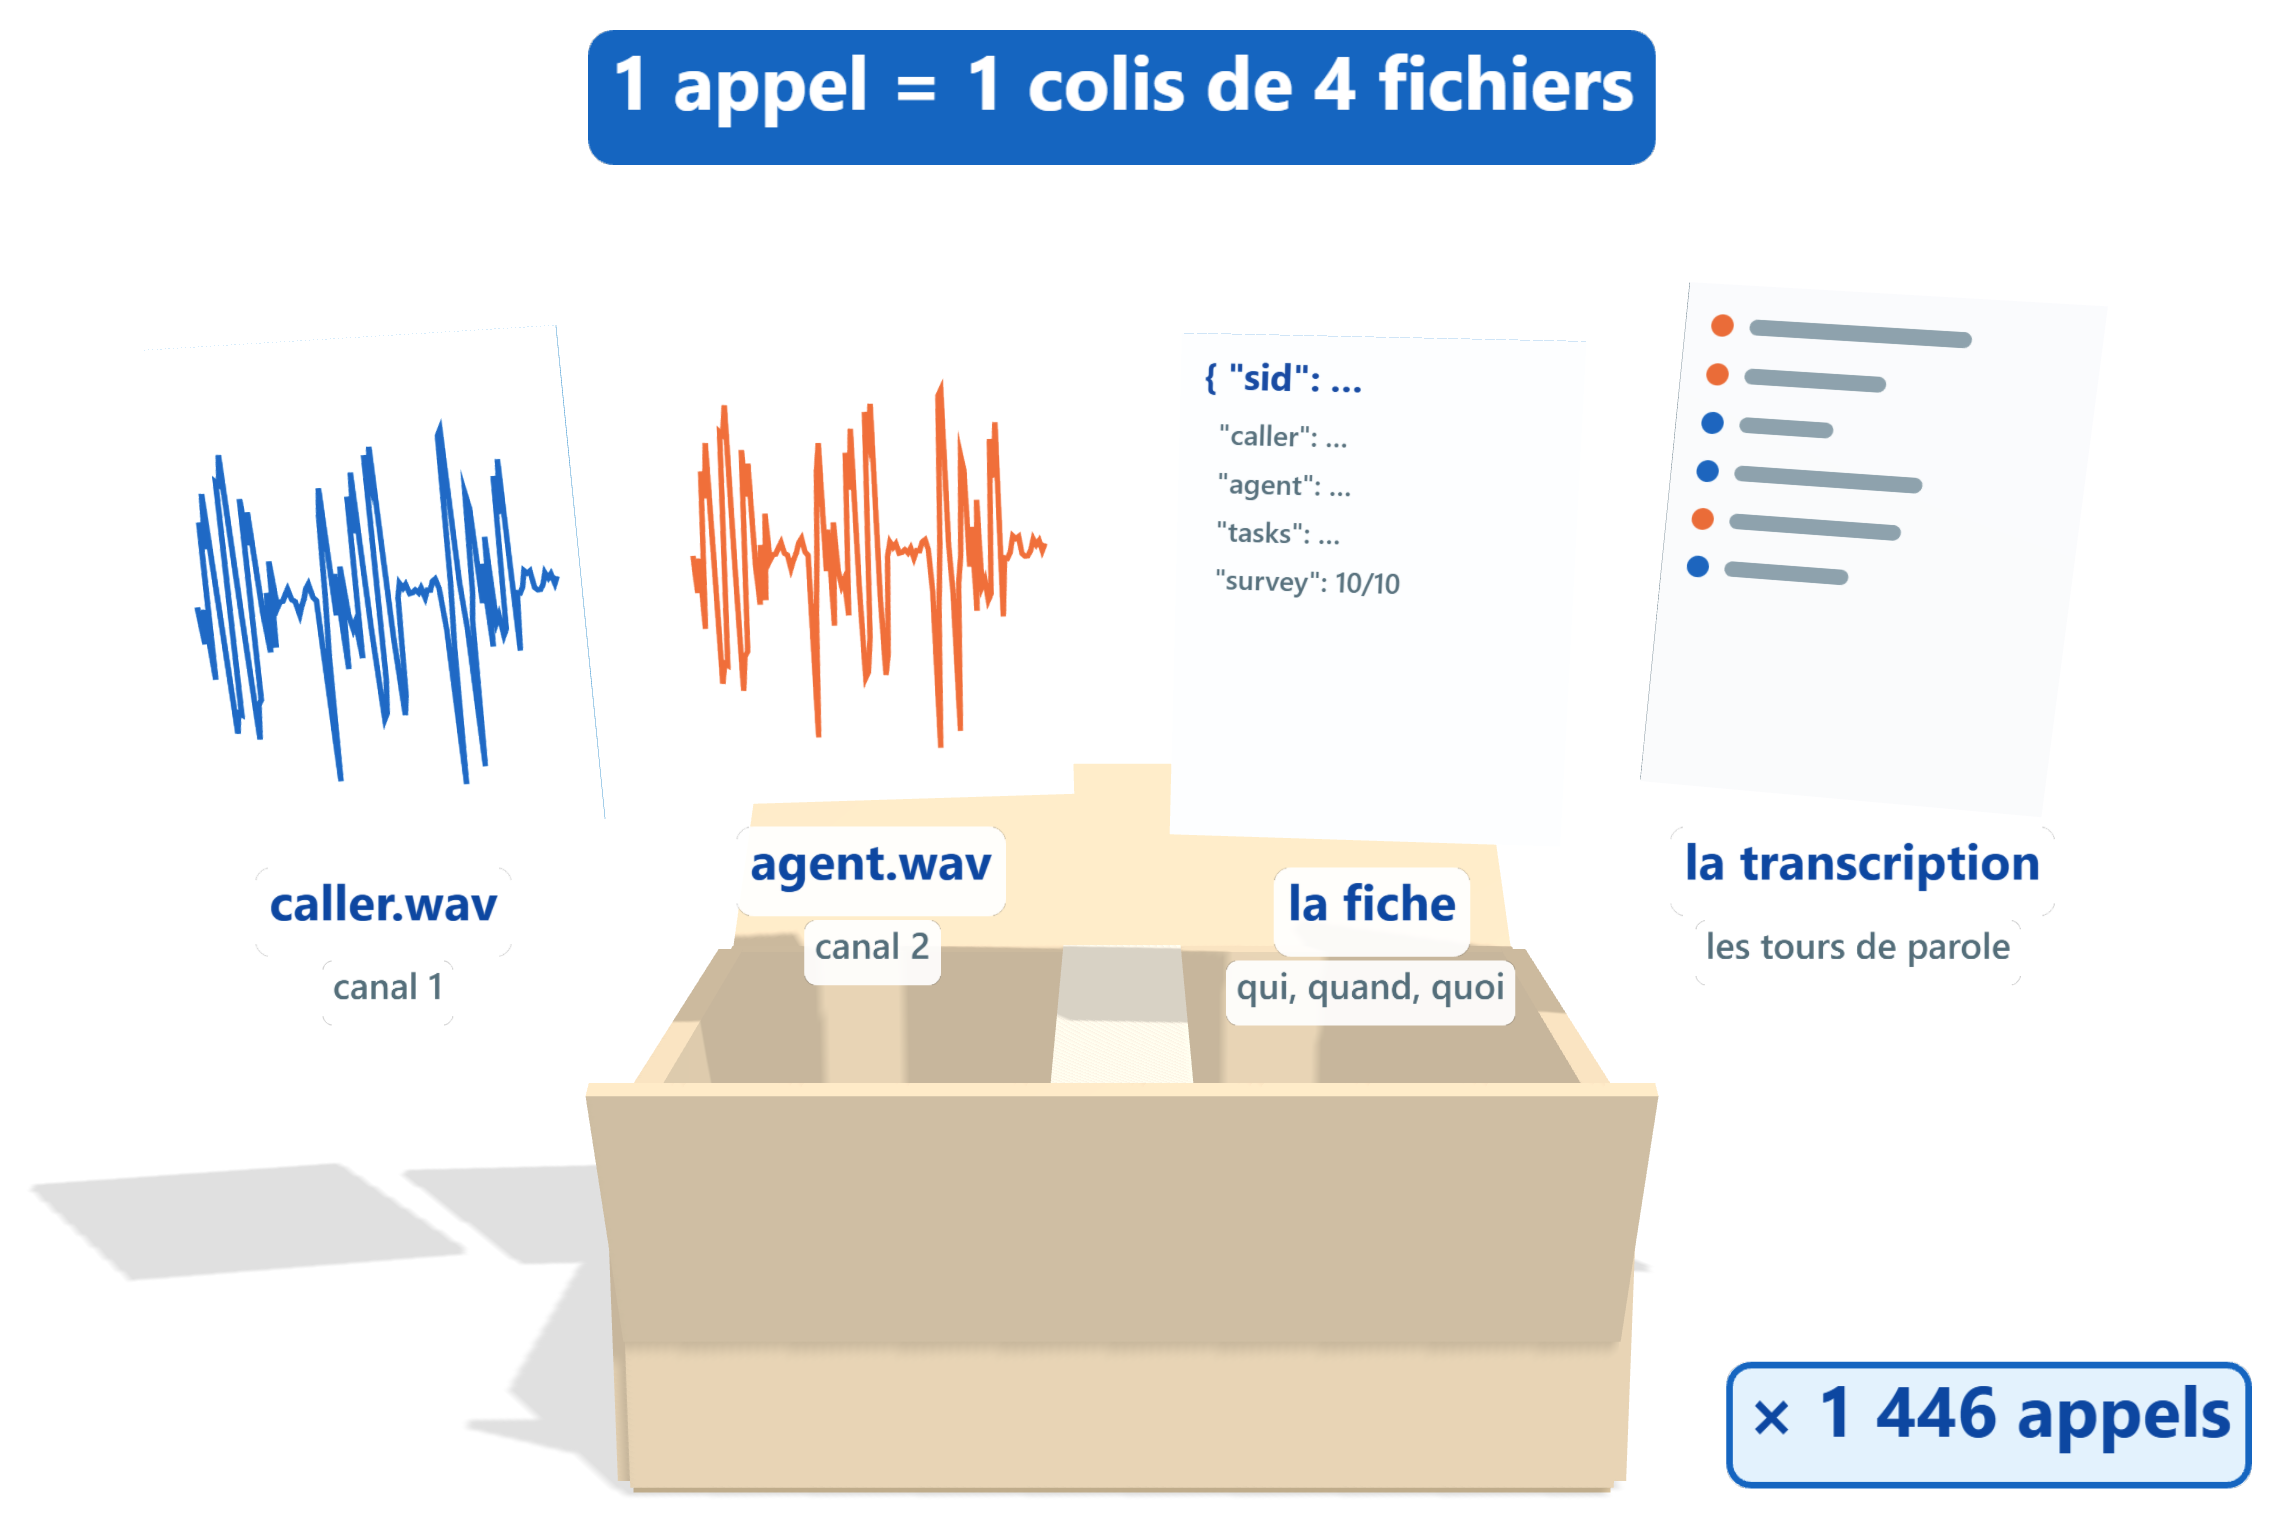
\includegraphics[width=0.68\linewidth]{3d_colis.png}
\end{center}

\begin{tcbraster}[raster columns=3, raster equal height, raster column skip=6pt, raster every box/.style={unbreakable}]
\begin{kpibox}[title={\faHeadphones\ Un canal}, unbreakable]
\small une ligne enregistrée à part : canal 1 = client, canal 2 = conseiller (en principe).
\image{deux talkies-walkies, deux cassettes}
\end{kpibox}
\begin{kpibox}[title={\faComments\ Un tour}, unbreakable]
\small un moment où une seule personne parle.
\image{chacun son tour d'avoir la balle}
\end{kpibox}
\begin{kpibox}[title={\faWind\ Un faux tour}, unbreakable]
\small un souffle ou un clic détecté comme un tour : \texttt{[noise]}.
\image{la lampe qui s'allume quand passe un chat}
\end{kpibox}
\end{tcbraster}

\begin{stepbox}[title={1.1\quad Deux tables : \texttt{appels} (1 ligne par appel) et \texttt{tours} (1 ligne par tour)}]
\doisvoir{}
\begin{center}
\cle{1\,446}{appels}\hspace{3pt}\cle{25\,730}{tours}\hspace{3pt}\cle{56 s}{médiane d'un appel}\hspace{3pt}\cle{9 s}{d'attente (médiane)}\hspace{3pt}\cle{55}{clients}
\end{center}
\end{stepbox}

\begin{stepbox}[title={1.2\quad Le client est-il toujours sur le canal 1 ?}]
Pour chaque appel : le canal le plus fréquent des tours du client. Compte ceux qui ne sont pas 1.
\doisvoir{\textbf{37 appels inversés.} Ce n'est pas ton code : c'est dans la base.}
\end{stepbox}

\begin{stepbox}[title={1.3\quad Les deux horloges : l'exercice le plus important}]
\begin{center}
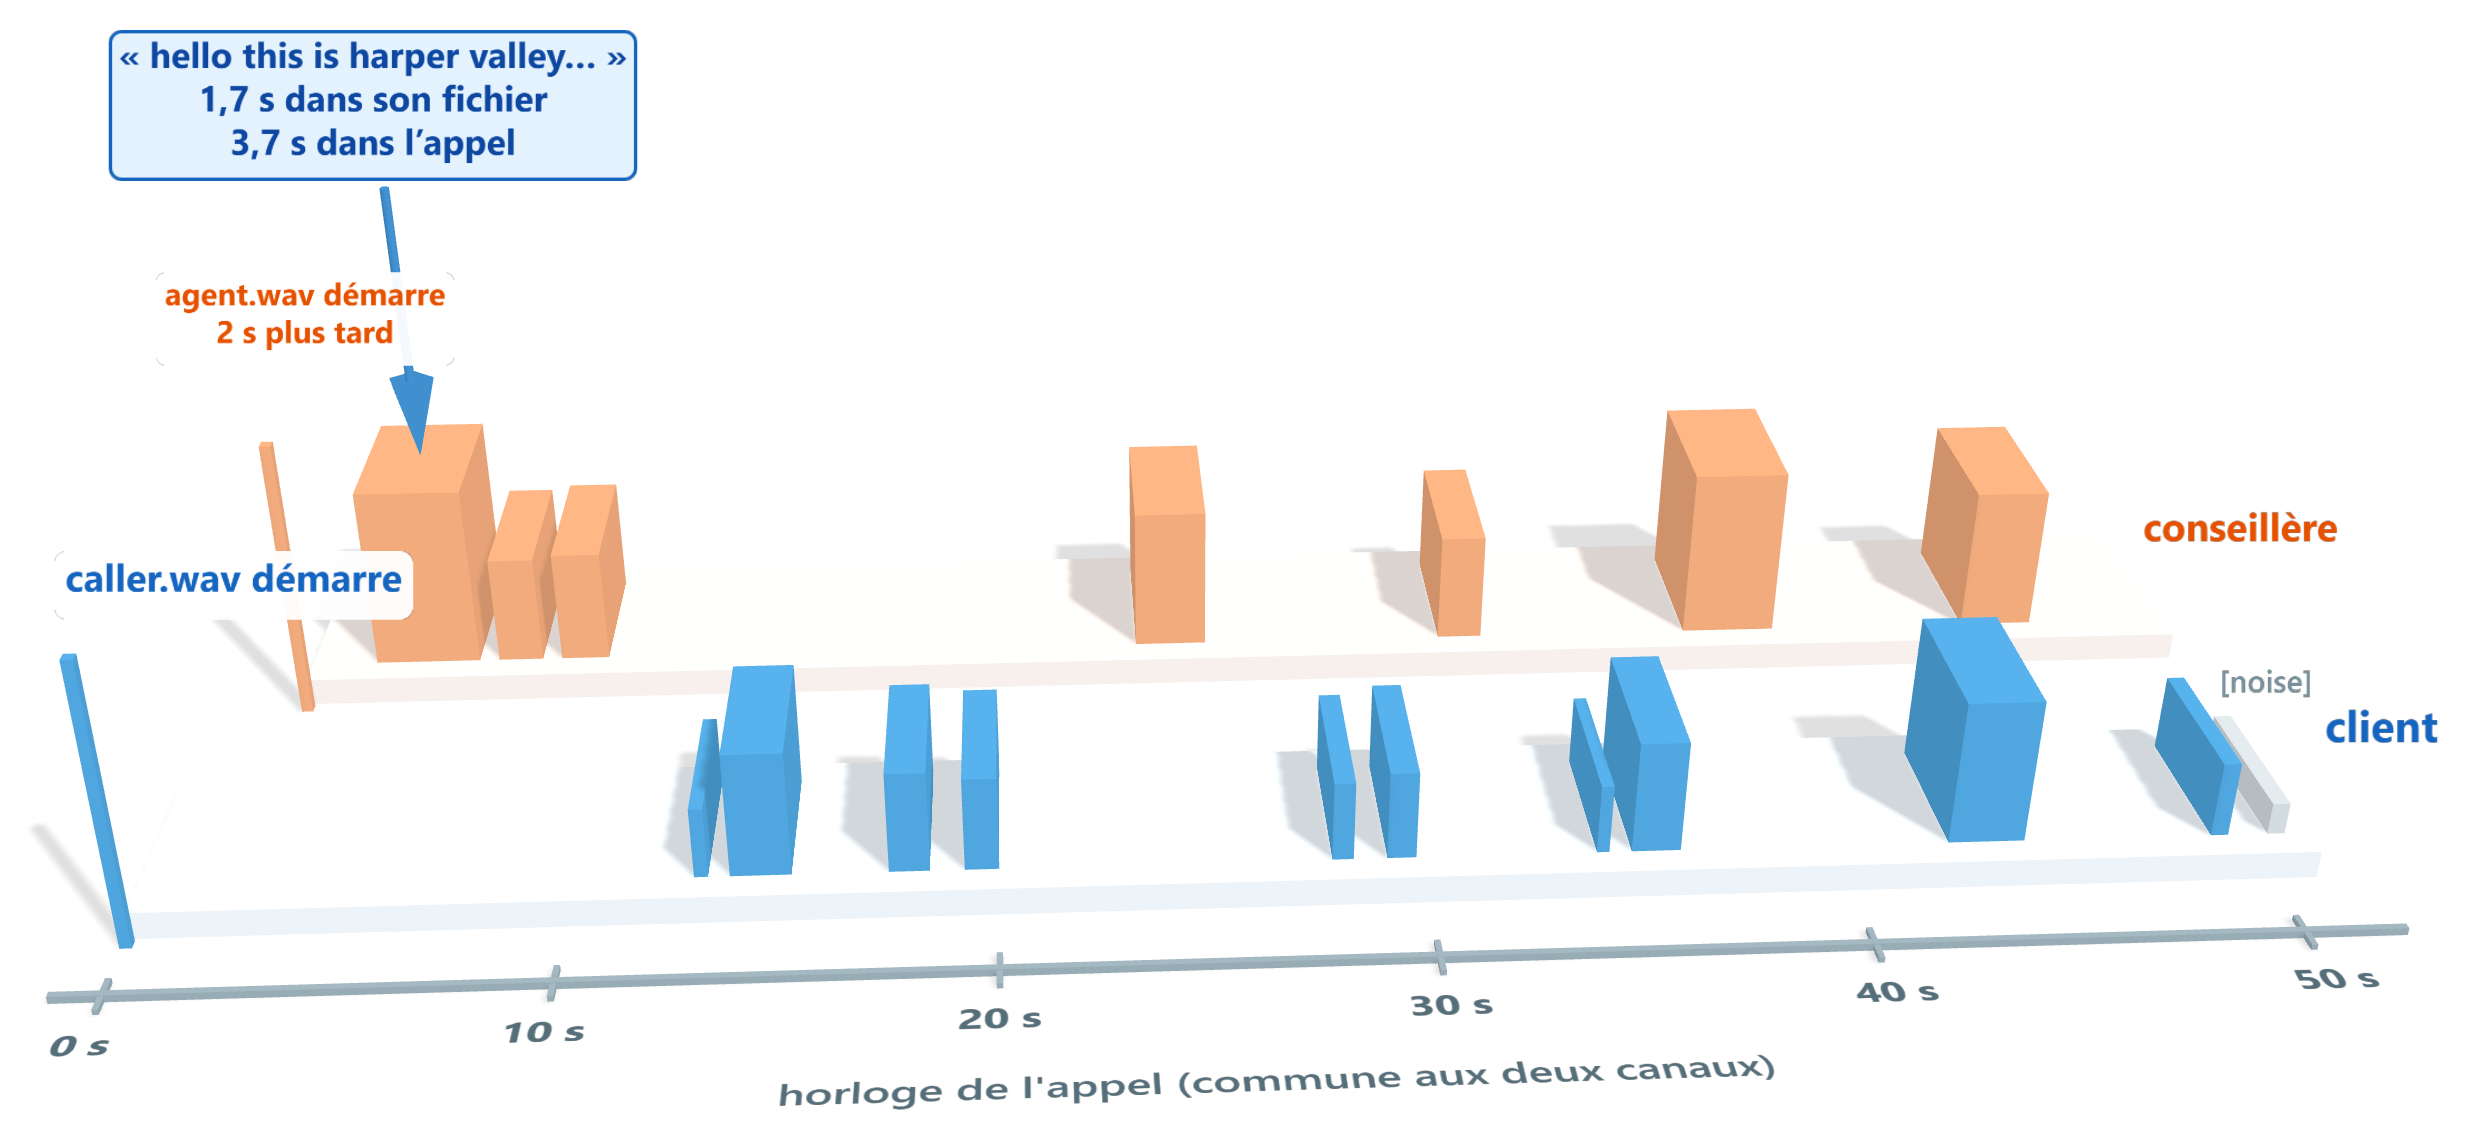
\includegraphics[width=\linewidth]{3d_pistes.png}
\end{center}
\begin{tcbraster}[raster columns=2, raster equal height, raster column skip=6pt, raster every box/.style={unbreakable}]
\begin{conceptbox}[title={\faFileAudio\ \texttt{position\_s} : où est la voix \textbf{dans son fichier}}]
pour \textbf{découper} l'audio (branche B)\\
\faArrowRight\ c'est \texttt{start\_ms}
\end{conceptbox}
\begin{conceptbox}[title={\faClock\ \texttt{debut\_s} : quand \textbf{dans l'appel}}]
pour \textbf{ordonner} les tours (branche C)\\
\faArrowRight\ c'est \texttt{offset\_ms}
\end{conceptbox}
\end{tcbraster}
\image{deux chronomètres : celui de la conseillère est lancé 2 secondes après celui de la cliente.}
\doisvoir{écart médian de \textbf{2,01 s} sur le canal 2, 0 sur le canal 1 ; la voix est à
\texttt{start\_s} dans \textbf{96 \%} des 1\,000 tours testés.}
\end{stepbox}

\begin{piege}
\textbf{C'est l'inverse de ce que dit la documentation.} En la croyant, tu découpes le conseiller
2~s trop tard dans 70~\% des appels, et ton code ne t'affiche \textbf{aucune erreur}.
\end{piege}

\begin{stepbox}[title={1.4\quad Dans quel fichier est la voix du client ?}]
Dans les 37 appels inversés, mesure l'énergie de chaque tour du client dans \texttt{caller} et dans
\texttt{agent}. Le fichier le plus fort contient sa voix.
\doisvoir{\textbf{162 tours testés}, \texttt{agent} plus fort dans \textbf{89 \%} des cas.}
\begin{center}
\begin{tikzpicture}[r/.style={draw=sectioncolor, fill=notebg, rounded corners=5pt, minimum height=1cm, align=center, font=\small, text width=6.6cm}]
\node[r] (a) {\textbf{Règle :} le fichier se choisit par le \textbf{canal},\\le rôle se lit dans la transcription.};
\node[right=0.4cm of a, align=left, font=\small] {\texttt{canal 1} \faArrowRight\ \texttt{caller/}\\\texttt{canal 2} \faArrowRight\ \texttt{agent/}};
\end{tikzpicture}
\end{center}
\image{deux tiroirs avec des étiquettes collées à l'envers : on ouvre et on regarde.}
\end{stepbox}

\begin{stepbox}[title={1.5\quad Regarde et écoute (rien à coder)}]
Change \texttt{sid\_exemple} (\texttt{appels.index[10]}, \texttt{[200]}\ldots) et écoute l'autre canal.
\faEye\ Toutes les zones colorées contiennent-elles de la parole ?
\end{stepbox}

\begin{stepbox}[title={1.6\quad Nettoyer et écarter le bruit}]
\texttt{nettoyer} : minuscules, sans \texttt{[balises]} ni \texttt{<unk>}, seulement lettres,
apostrophe, espaces. \texttt{parole} = la transcription \textbf{automatique} nettoyée n'est pas vide.
\doisvoir{\textbf{14,4 \%} des tours du client sans parole.}
\end{stepbox}

\section{Partie 2 : l'étiquette}

\begin{formulabox}
\centering\large $\text{valence} = p_{\text{pos}} - p_{\text{neg}}$ \qquad
\faArrowRight\qquad $y = 1$ si l'appel est dans le \textbf{quart le plus bas}
\end{formulabox}

\begin{enfant}
\textbf{Un thermomètre d'humeur, pas l'humeur.} $y=1$ ne veut pas dire \og client mécontent \fg{},
mais \og l'outil l'a trouvé moins positif que les autres \fg{}.
\end{enfant}

\begin{stepbox}[title={2.1 à 2.4\quad Construire, puis auditer l'étiquette}]
\begin{tabularx}{\linewidth}{>{\bfseries\color{sectioncolor}}c X >{\raggedright\arraybackslash}p{4.6cm}}
2.1 & construire \texttt{valence}, \texttt{valence\_client}, \texttt{seuil}, \texttt{y} & \faCheckCircle\ seuil \textbf{0,039} ; \textbf{362} appels à 1 \\
2.2 & lire les 15 tours les plus négatifs et les 15 plus positifs & \faCheckCircle\ \textbf{3\,322} tours candidats \\
2.3 & part de $y=1$ par motif et par client & \faCheckCircle\ \textbf{8} motifs, \textbf{45} clients \\
2.4 & la même phrase \og hi my name is\ldots \fg{} selon le nom & \faCheckCircle\ \textbf{386} présentations \\
\end{tabularx}
\end{stepbox}

\begin{center}
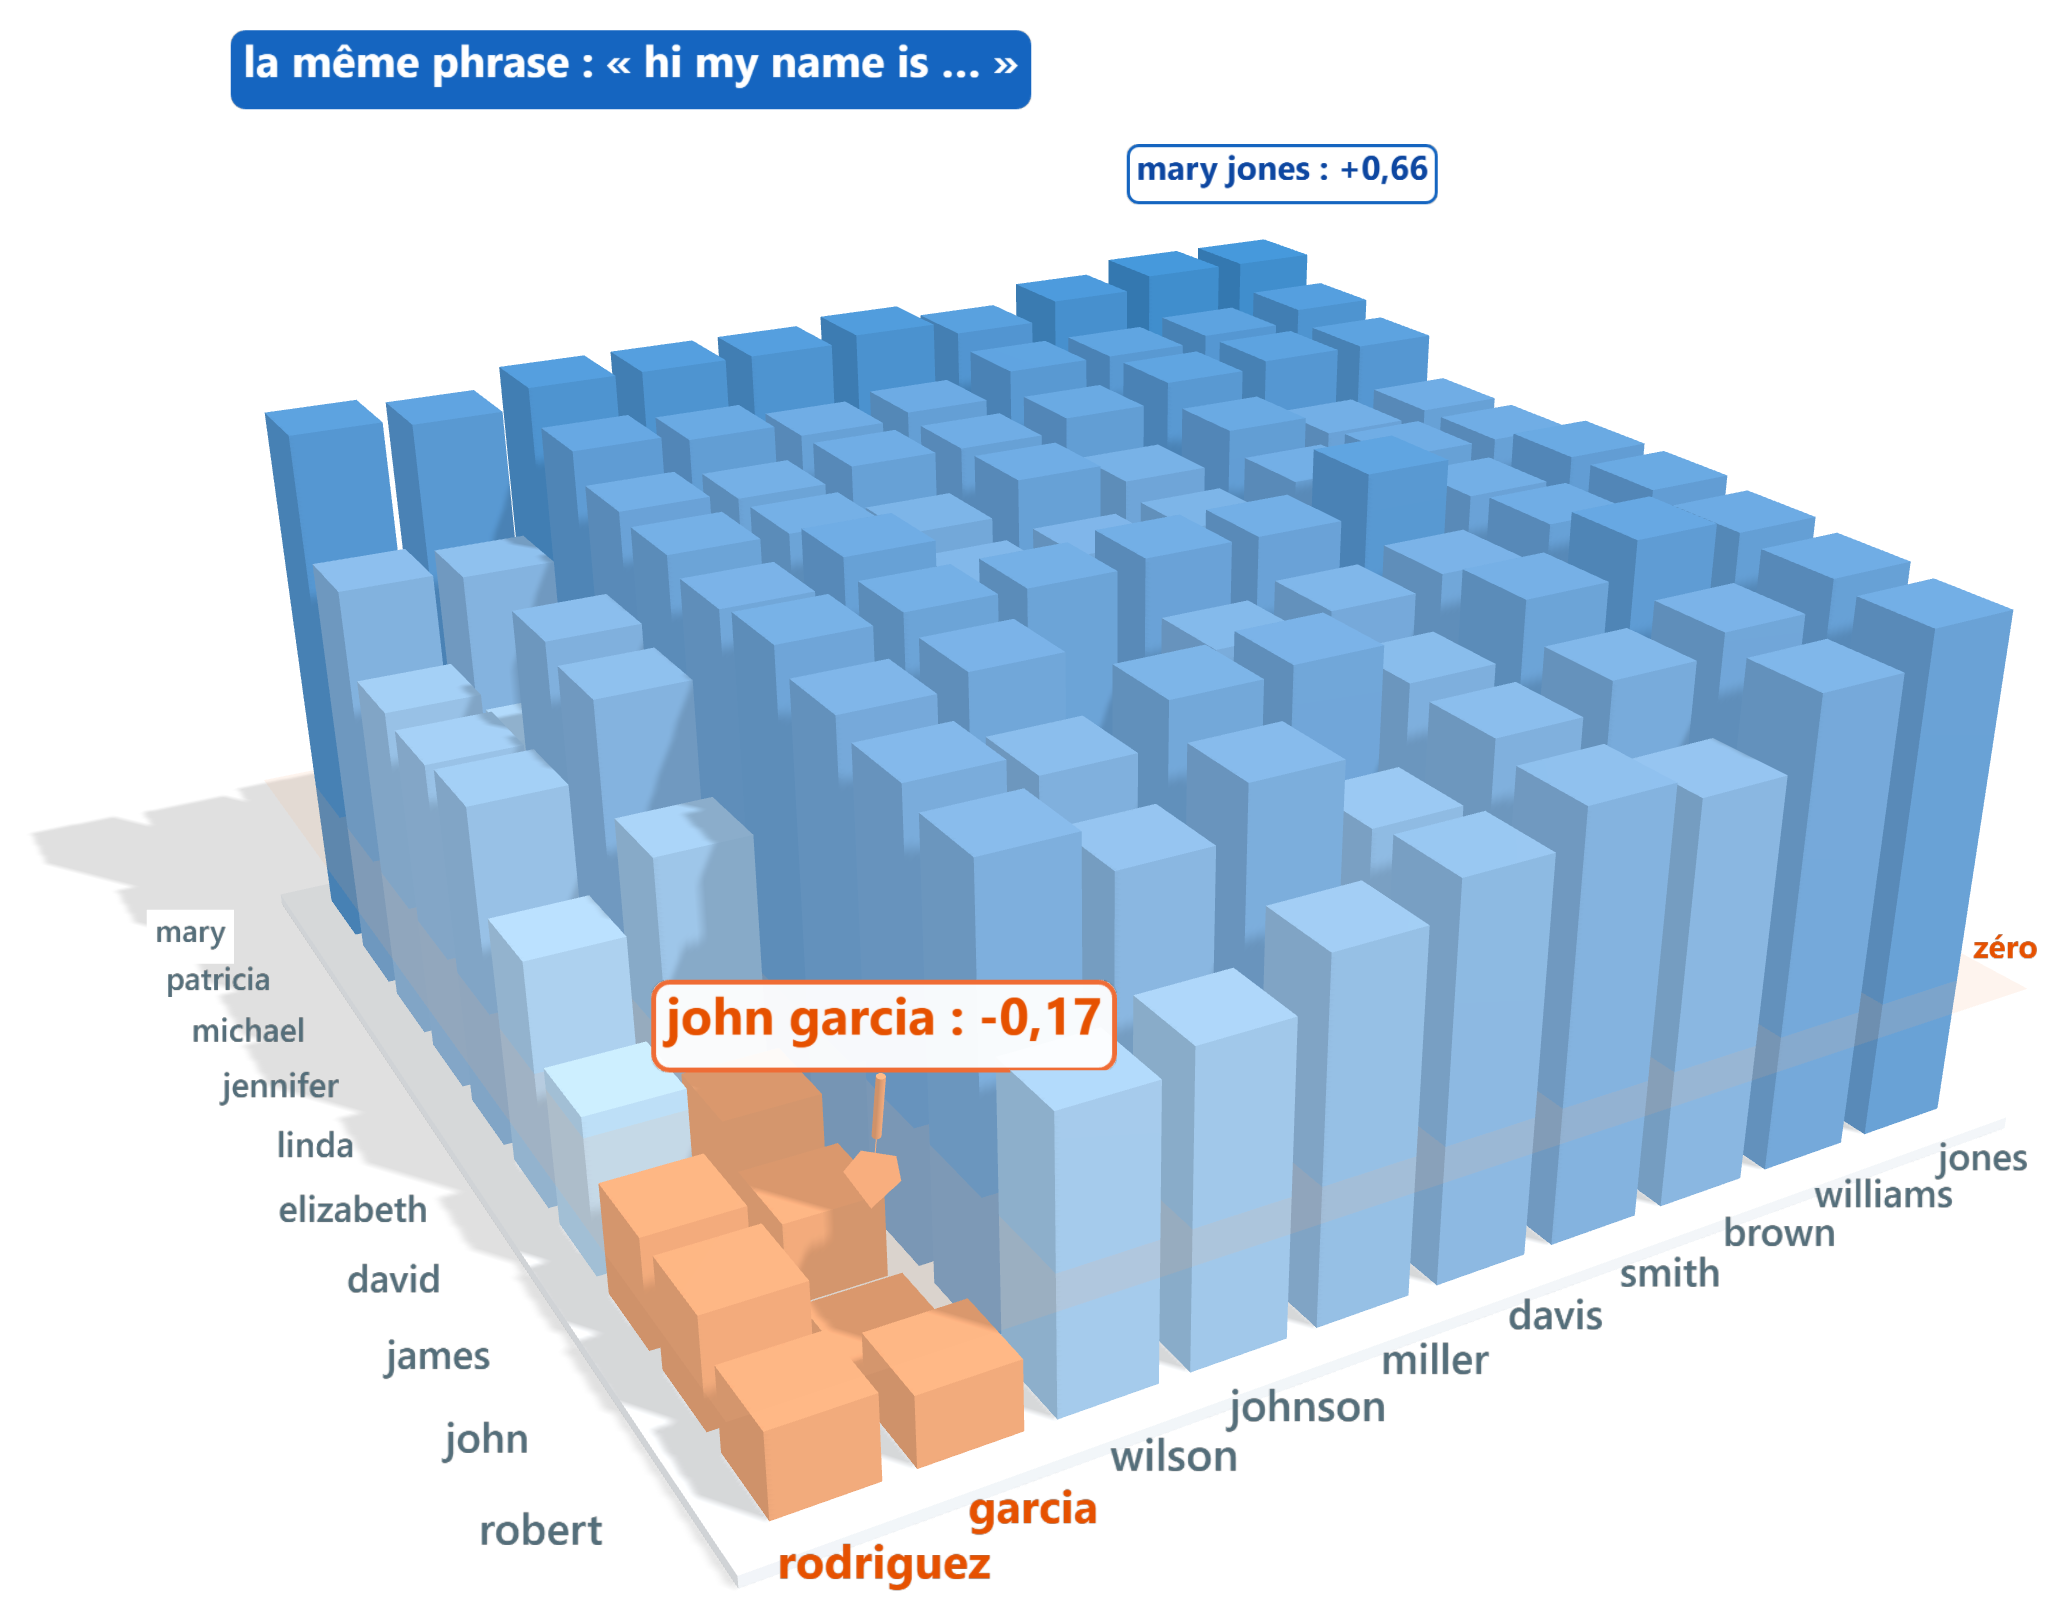
\includegraphics[width=0.66\linewidth]{3d_grille.png}
\end{center}

\begin{piege}
\textbf{La même phrase, deux notes.} \og John Garcia \fg{} : $-0{,}17$. \og Mary Jones \fg{} :
$+0{,}66$. Le nom change la note de l'outil. \faArrowRight\ On \textbf{anonymise avant} tout outil
de sentiment.\par\smallskip
\textbf{Retiens :} un nom dans le texte, même celui d'un personnage fictif, devient un biais. Dans notre
projet, on masque les noms \textbf{dès le départ} : \texttt{[nom]} pour tout le monde.
\end{piege}

\clearpage
\section{Partie 3 : mesurer sans tricher}

\begin{center}
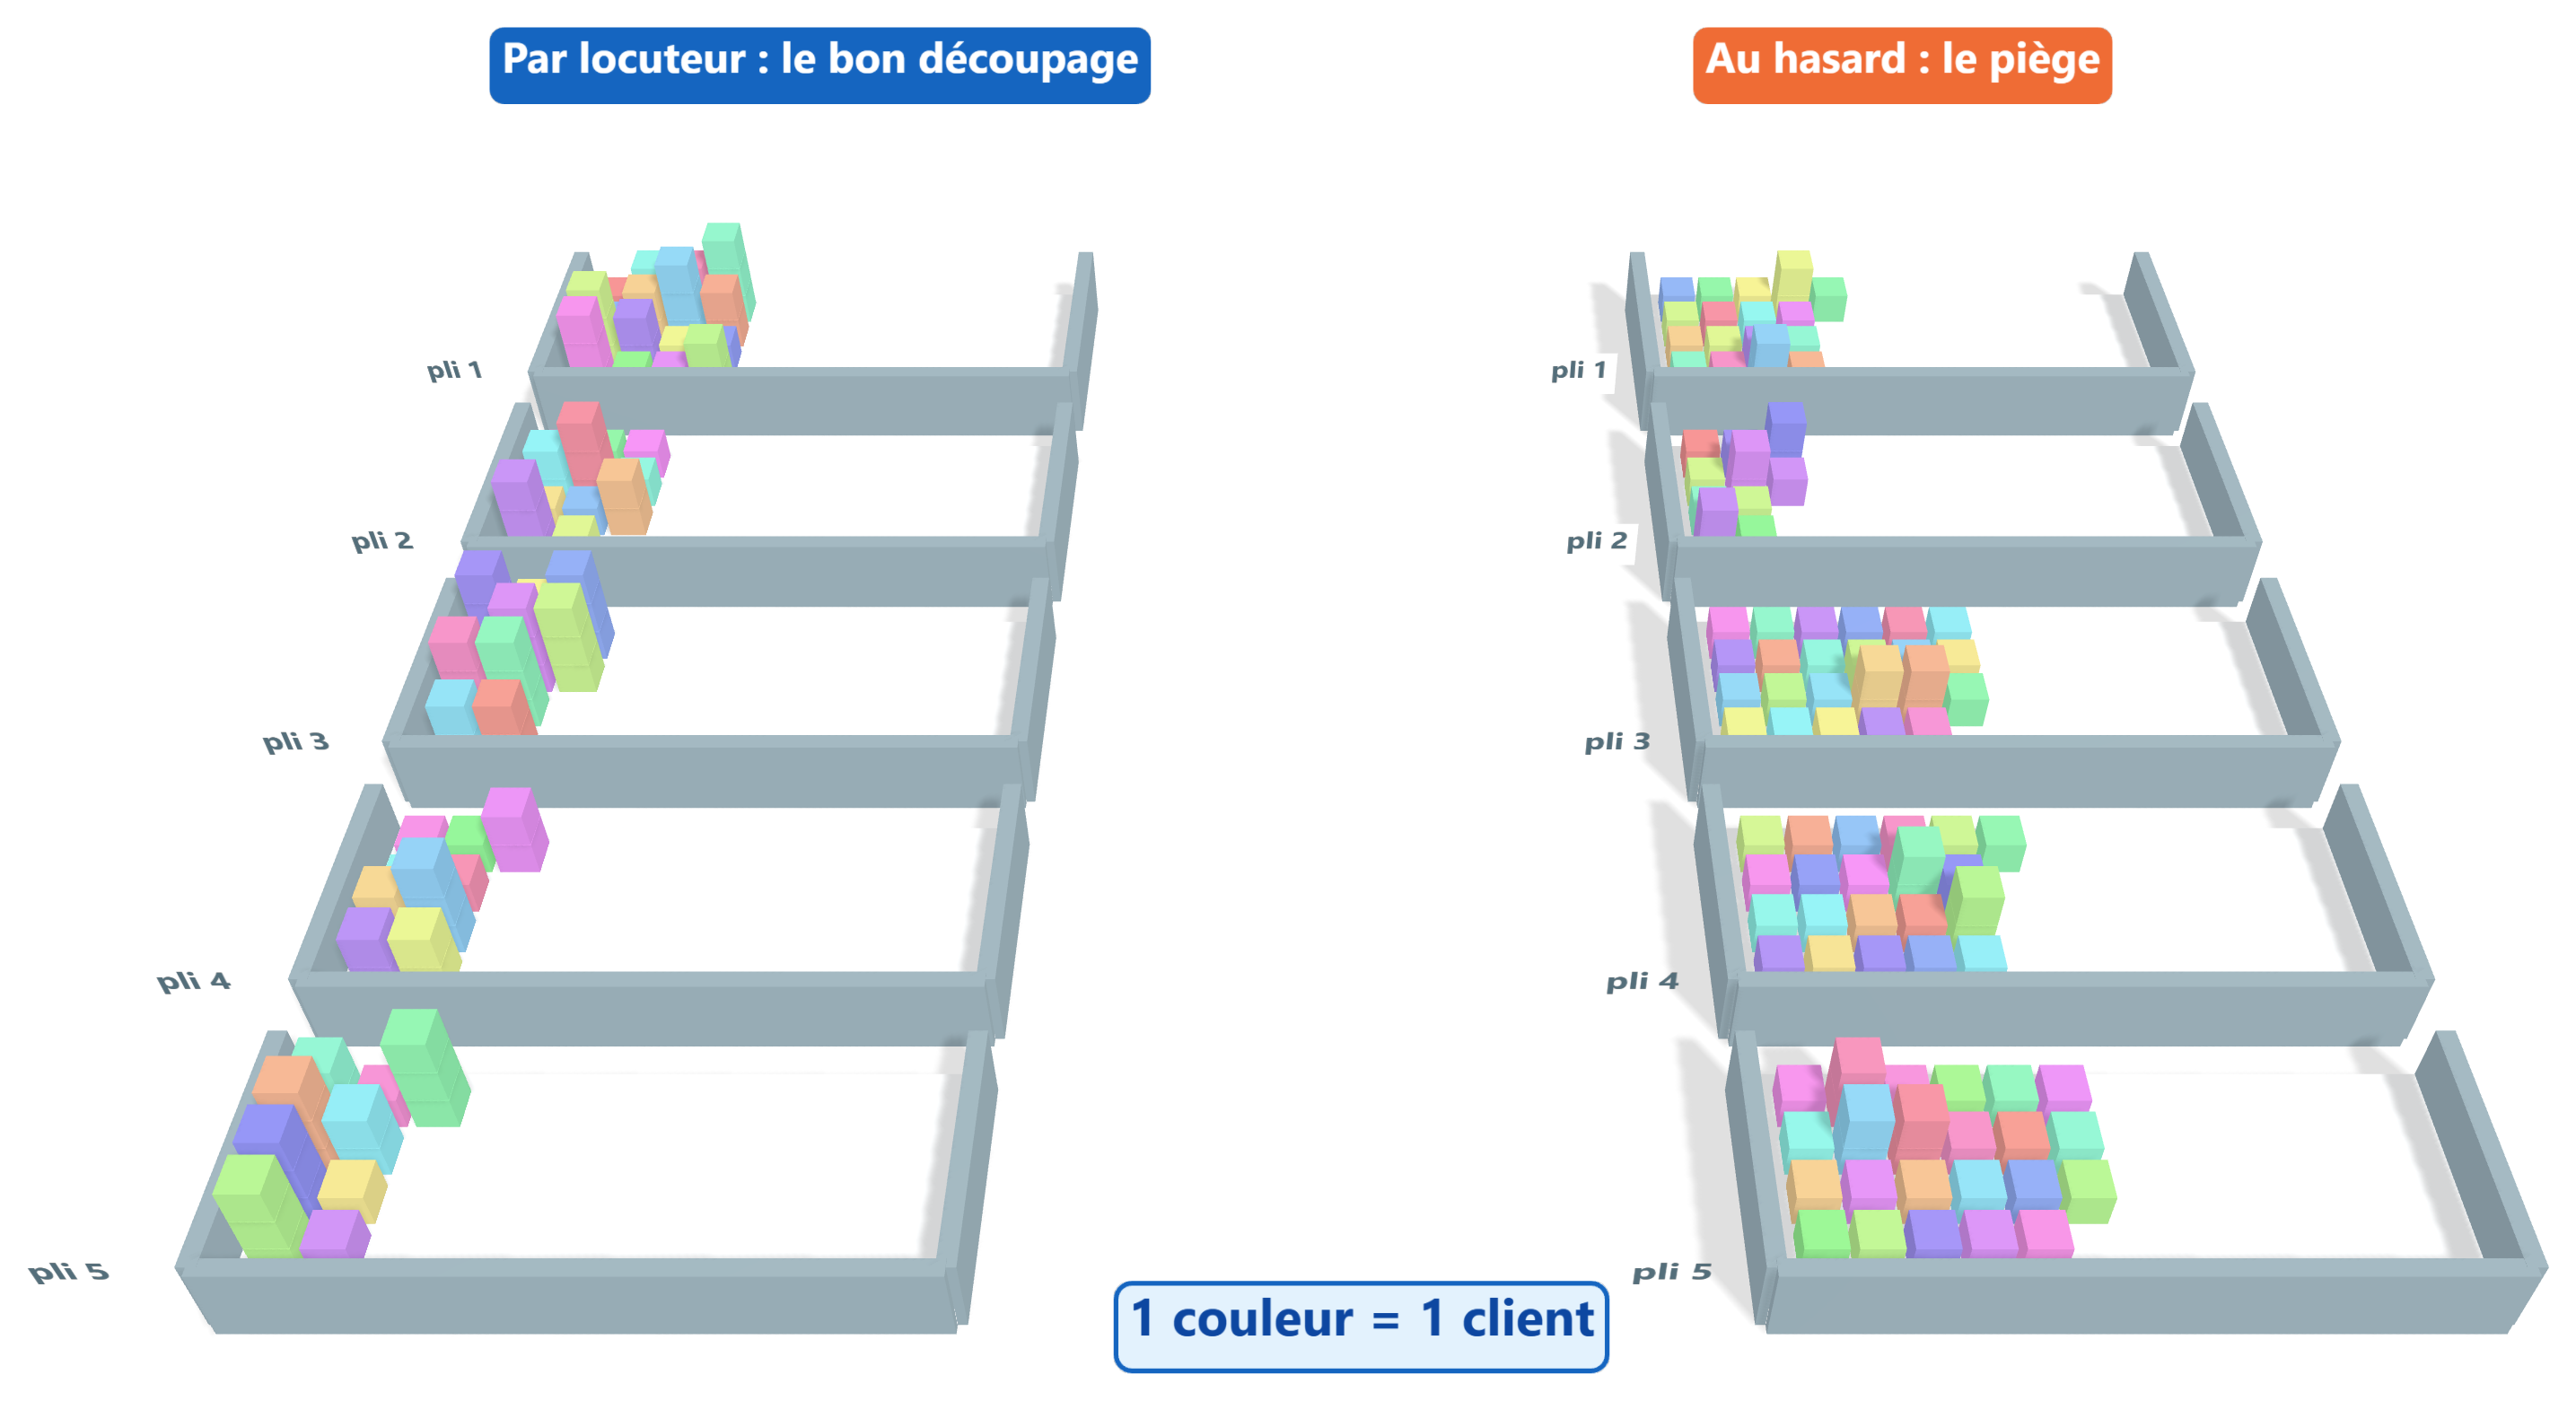
\includegraphics[width=0.92\linewidth]{3d_plis.png}
\end{center}

\begin{enfant}
\textbf{Examen et révisions} : à l'examen, pas d'exercices de la même personne qu'en révision,
sinon on reconnaît l'écriture au lieu de comprendre. Ici : \textbf{tous les appels d'un client du
même côté}.
\end{enfant}

\begin{center}
\begin{tikzpicture}[x=1.3cm, y=0.55cm]
\foreach \e in {0,...,4} {
  \node[anchor=east, font=\small] at (-0.15,-\e) {expérience \e};
  \foreach \p in {0,...,4} {
    \ifnum\p=\e
      \fill[orange!80!red] (\p,-\e-0.4) rectangle (\p+0.95,-\e+0.4);
      \node[font=\scriptsize\bfseries, color=white] at (\p+0.475,-\e) {test};
    \else
      \fill[sectioncolor!70] (\p,-\e-0.4) rectangle (\p+0.95,-\e+0.4);
    \fi
  }
}
\node[anchor=west, font=\small, text width=5.2cm] at (5.2,-2) {\faArrowRight\ chaque appel est testé \textbf{une fois}, par un modèle qui ne l'a jamais vu : ce sont les \textbf{scores hors pli}};
\end{tikzpicture}
\end{center}

\begin{stepbox}[title={3.1\quad Les plis}]
\begin{lstlisting}
plis = list(StratifiedGroupKFold(n_splits=5, shuffle=True, random_state=0)
            .split(appels, y, groups=appels.id_client))
\end{lstlisting}
\doisvoir{5 plis de \textbf{273 à 321} appels, \textbf{9 à 16} clients chacun, aucun client des deux côtés.}
\end{stepbox}

\begin{tcbraster}[raster columns=2, raster equal height, raster column skip=8pt, raster every box/.style={unbreakable}]
\begin{kpibox}[title={\faTrophy\ AUC}, unbreakable]
On tire un appel à 1 et un appel à 0 : chance que le modèle classe le 1 plus haut.\\
\textbf{0,5} = pile ou face \quad \textbf{1} = parfait
\image{le jeu des deux enveloppes}
\end{kpibox}
\begin{kpibox}[title={\faListOl\ Précision moyenne}, unbreakable]
Regarde surtout le \textbf{haut de la liste} : les appels qu'on remonterait à un superviseur.\\
\textbf{0,25} = hasard
\end{kpibox}
\end{tcbraster}

\begin{stepbox}[title={3.2\quad Le repère à battre : le motif seul}]
\doisvoir{}
\begin{center}
\cle{0,637}{AUC}\hspace{8pt}\cle{0,349}{précision moyenne}
\end{center}
\end{stepbox}

\begin{piege}[unbreakable]
\textbf{Ta barre, c'est 0,637, pas 0,5.} Une branche à 0,62 n'a rien appris : le motif seul fait
mieux.
\image{deviner la météo en disant \og comme aujourd'hui \fg{} : le vrai météorologue doit faire mieux.}
\end{piege}

\begin{conceptbox}[title={La barre \og motif seul \fg{} que tu verras avant la branche A}, unbreakable]
\small Ce n'est pas une branche. C'est un modèle qui ne connaît que la raison de l'appel (\og pay bill \fg{},
\og get branch hours \fg{}\ldots), recalculé dans les mêmes plis et posé à côté des branches pour servir
de ligne de lecture. Il atteint 0,637 parce que certains motifs sont plus pénibles que d'autres : 47\,\%
d'appels étiquetés~1 pour \og pay bill \fg{}, 11\,\% pour \og get branch hours \fg{}.
\begin{center}
\begin{tikzpicture}[x=26cm, y=1cm, font=\footnotesize]
\fill[slate!12] (0.45,-0.35) rectangle (0.637,0.35);
\fill[notebg] (0.637,-0.35) rectangle (0.91,0.35);
\draw[thick, ->] (0.45,0) -- (0.915,0) node[right] {AUC};
\foreach \v/\l in {0.5/0{,}5, 0.6/0{,}6, 0.7/0{,}7, 0.8/0{,}8, 0.9/0{,}9} \draw (\v,-0.07) -- (\v,0.07) node[pos=0, below=8pt] {\l};
\draw[very thick, darkblue] (0.637,-0.65) -- (0.637,0.65) node[pos=0, below=2pt, font=\footnotesize\bfseries] {motif seul 0,637};
\foreach \v/\n/\c in {0.526/{B, 0,526}/sectioncolor, 0.614/{C, 0,614}/slate, 0.849/{A, 0,849}/accentblue}
  \fill[\c] (\v,0) circle (2.8pt) node[above=6pt, font=\footnotesize\bfseries, color=\c] {\n};
\end{tikzpicture}
\end{center}
À gauche de la ligne : la branche n'a rien appris de plus que le motif. À droite : elle apporte de
l'information sur la tonalité.
\end{conceptbox}

\begin{tcolorbox}[colback=titlebg, colframe=titlebg, coltext=white, arc=5pt, boxrule=0pt,
  left=15pt, right=15pt, top=10pt, bottom=10pt]
\begin{center}
{\Large\bfseries En fin de séance, tu as :}\\[8pt]
\begin{tabular}{c c c}
{\huge\faTable} & {\huge\faTag} & {\huge\faBalanceScale} \\[4pt]
\textbf{2 tables propres} & \textbf{1 étiquette} & \textbf{1 protocole} \\
\texttt{appels}, \texttt{tours} & dont tu connais les défauts & plis par client, repère 0,637 \\
\end{tabular}
\end{center}
\end{tcolorbox}
